\documentclass{article}

\linespread{1.5}
\usepackage[utf8]{inputenc}
\usepackage[left=1.35in,right=1.35in,bottom=1in]{geometry}
\setlength\parindent{0pt}
\setlength{\parskip}{1em}
\setcounter{secnumdepth}{0}
\usepackage{outlines}
\usepackage{graphicx}
\graphicspath{ {imgs} }
\usepackage[hyphens]{url}
\usepackage{hyperref}
\usepackage{color,soul}
\usepackage[normalem]{ulem}
\usepackage{tabularx}
\usepackage{pgfgantt}

\usepackage[
backend=biber,
style=apa,
citestyle=authoryear,
sorting=nyt,
]{biblatex}
\addbibresource{refs.bib}

\usepackage{comment}
\specialcomment{topicsen}{\begingroup\bfseries\scriptsize}{\endgroup}
%\excludecomment{topicsen}

\newcommand{\alignedmarginpar}[1]{%
        \marginpar{\raggedright\small #1}
    }
    
\newcommand{\bisection}[1]{\textbf{\textit{#1}}}

\DeclareCiteCommand{\citeyear}
    {}
    {\bibhyperref{\printdate}}
    {\multicitedelim}
    {}

\title{Research Proposal}
\author{Carla Hyenne}
\date{}

\begin{document}

\maketitle

\tableofcontents 

%%%%%%%%%%%%%%%%%%%%%%%%%%%%%%%%%%%%%%%%%%%
%				ABSTRACT (MAX 500 WORDS)
%%%%%%%%%%%%%%%%%%%%%%%%%%%%%%%%%%%%%%%%%%%
\pagebreak
\section{Abstract}

The benefits of urban nature on people’s health, for fostering community, and for climate change adaptation are widely acknowledged. Within the discourse of environmental justice (EJ), these benefits have been used to demonstrate that equitable access to healthy, unpolluted environments is a human right, with scholars like Anguelovski and Agyeman arguing that marginalised and vulnerable populations are disproportionately affected by lack of access to such spaces. 

Despite extensive studies on the accessibility of urban green spaces (UGS), urban blue spaces (UBS) have not been given the same attention. Moreover, research on UGS accessibility has focused on geographical accessibility, such as proximity to home, and has seldom considered subjective experiences as influencing access. However, accessibility is a multidimensional and complex concept which cannot be reduced to spatial distribution. As Wang, Brown and Liu put forward, perceived accessibility that addresses subjectivities, socio-personal characteristics, and the quality and diversity of the space, must also be considered.

My research addresses the issue of perceived accessibility to UBS by looking at the extent to which subjective experiences and perceptions shape how (un)fairly accessible high-quality, public UBS interventions are, and what this means for the environmentally just city.
I will pay special attention to socio-economic and personal characteristics such as age, gender, income, ethnicity, cultural practices, and general preferences for infrastructure and aesthetics.

Specifically, I will be looking at three blue spaces in Copenhagen located in neighbourhoods with varying socio-economic and demographic profiles. A combination of observations of human activity, surveys with users, and interviews with experts will allow me to study a variety of perspectives on UBS. I will discuss the extent to which the city of Copenhagen offers equitable opportunities for people with different backgrounds and preferences to enjoy UBS, and juxtapose this against the ideal of the environmentally just city. 
Given the availability of UBS in Copenhagen and the importance the city is giving to harbour baths and urban beaches, it will be particularly useful to evaluate whether Copenhagen’s UBS caters to everyone’s needs.

I argue that perceived accessibility is an important dimension of EJ, because public UBS are places of community, attachment, and well-being. Ignoring subjective experiences that differ from the mainstream can contribute to social inequalities, discrimination, and displacement.

In conclusion, my research will closely examine how perceptions shape accessibility to UBS. It will serve to understand what perceptions and experiences those who control access (city planners) must take into account if UBS are to be usable by everyone.
% especially those of marginalised and vulnerable communities.

%%%%%%%%%%%%%%%%%%%%%%%%%%%%%%%%%%%%%%%%%%%%
%								LITERATURE REVIEW (2-3 PAGES)
%%%%%%%%%%%%%%%%%%%%%%%%%%%%%%%%%%%%%%%%%%%%
\pagebreak
\section{Literature review}

This section reviews the academic literature on urban blue spaces (UBS), and incorporates literature from wider fields like urban ecology. It also introduces concepts that are central for understanding equity with regards to UBS, namely environmental justice and accessibility. 
% These two concepts will be central to the research.

% Context and relevant background info - 2 paragraphs
\subsubsection{The benefits of urban blue spaces}

In an urban context, UBS have undeniable positive effects which Gascon et al. (\citeyear{gascon2017outdoor}) summarise as ``stress reduction, increased physical activity, promotion of positive social contacts, increased place attachment and the reduction of extreme temperatures''. These benefits fall under three broad categories: health and well-being, community, and climate adaptation.
First, being exposed to water makes people feel better, happier, and be more active. There is an extensive repertoire of quantitative studies demonstrating these effects on people's health and well-being (\cite{gascon2017outdoor}, \cite{britton2020blue}).
Qualitative studies also show that exposure to UBS improves mental health, regardless of how people interact with it (\cite{garrett2019urban}, \cite{van2021urban}).
Second, UBS give people the opportunity to connect with each other and with nature. UBS revitalisation projects can be an opportunity to create community bonds by engaging residents in the design and implementation process. For example, the small-scale waterfront intervention in a deprived area of Plymouth, UK, revealed that residents who participated in the project reported a greater sense of well-being and life satisfaction due to feelings of community belonging and safety \parencite{van2021urban}.
Lastly, in the context of climate change, UBS can naturally alleviate pollution, heat stress, flooding or drought, and increase the climate resiliency of cities (\cite{lin2020water}, \cite{o2021international}). 

Given the potential of UBS, and that public space is highly valued commodity in the city, revitalising unused UBS into attractive environments helps make the most of all urban areas.
 
% Critical review, comparison, summary of literature - 1.5 pages
\subsubsection{The social and environmental consequences of blue urban renewal}

Despite the undeniable benefits of water in the city, transforming UBS into high-quality public space can have harmful consequences on people
% thesis --> add "and the environment" and clarify how improvements to UBS can harm environment
Two mechanisms of action are exclusionary planning, and neoliberal urban renewal. These reinforce socio-spatial inequalities by discriminating against people on the basis of socio-economic and cultural differences, or by way of racist and sexist practices.

% disrupting relationships
First, in contrast to the social bonds that can be fostered when residents are involved in revitalisation projects, connections between people and with nature can be disrupted if UBS are revitalised without considering the local community's perceptions. As Toomey et al. (\citeyear{toomey2021place}) demonstrate, people do attach meaning to degraded or polluted UBS, and it can't be assumed that these hold no value for the local community. 
% This is particularly susceptible to happen when a community's social practices do not fit with the social norms \parencite{wessells2014urban}. 
However, marginalised or stigmatised communities may find it hard to communicate their experience when consulted by planners, because they lack a common language to articulate their reality. And vice-versa: wealthy, white, males may not be capable of understanding the experience of `others' \parencite{anguelovski2020expanding}. To this end, Toomey et al. (\citeyear{toomey2021place}) propose using language like ``place-disruption'' and ``place-protection'' to promote mutual understanding and avoid privileging the values of mainstream groups over those of marginalised communities.

% neoliberal urban renewal
Second, cities are prioritising economic growth over well-being and community. Local governments are exploiting nature-based solutions to brand their cities as green and liveable,
% grave --> \footnote{For example, Madrid promoting the Madrid Río project on the official tourism website \parencite{madridrio}, or Oslo advertising its new urban waterfront promenade along which ``you find yourself surrounded by some of Oslo's world-renowned architectural gems'' \parencite{visitoslo}.}
and to promote greening (which includes blue space) as a win-win strategy where ``no one is left behind by the trickle-down of benefits from green infrastructure'' \parencite{anguelovski2021green}.
Anguelovski et al. (\citeyear{anguelovski2021green}) explain that with ``glitzy green'' renewal projects, cities try to attract a new creative class rather than addressing public UBS as a common good and prioritising the concerns of existing residents (\cite{wessells2014urban}, \cite{anguelovski2020expanding}).
These strategies perpetuate inequalities by privileging the values of white, environmentally privileged upper classes who can afford to live near nature. This phenomenon is referred to as green gentrification, where upgrading green space causes the exclusion and displacement of residents, who are priced out to a neighbourhood with less attractive nature. Given the similarities in benefits and attractivity of living near blue space, it is not farfetched to assume that \textit{blue gentrification} also takes place.


\subsubsection{The environmental justice principle}

To articulate the phenomenon whereby natural spaces provide social and environmental benefits but at the same time discriminate against vulnerable populations, scholars have used the concept of environmental justice (EJ).
EJ has evolved into the principle that everyone should have equal opportunities to access clean, healthy, unpolluted spaces, and in turn, share environmental burdens. As Agyeman et al. explain (\citeyear{agyeman2016trends}), it started as a social movement in the US in the 1980s at a time when it became obvious that ethnic minority and low-income populations were disproportionately exposed to polluted and degraded land.

Since then, EJ has concretised into an academic discourse and is typically broken down into three categories: distributional justice, procedural justice, and recognition justice.
Applied to public blue-green space (BGS), distributional justice refers to where these are situated in the city.
Procedural justice deals with questions of discrimination in public participation and decision making. 
Recognition justice addresses individual and community perceptions and preferences which may influence how people interact, or not, with the space.

% thesis -->  argue that sustainability not being only enviro but also eco and social, and \parencite{agyeman2016trends}
% grave --> environmental justice is concerned with whether social, economic, racial or ethnic inequalities are addressed and by striving to ``avoid displacement and new negative green, ecological, climate and health effects'' \parencite{anguelovski2020expanding}.

The applications of EJ on blue spaces are limited in comparison to green space. One study that stands out is Raymond et al.'s (\citeyear{raymond2016integrating}) research on the diversity of people, activities and perceived unpleasant experiences in Helsinki's blue spaces. The wide range of opinions they find show the importance of considering a multitude of perceptions when planning UBS, because people of different age, income, gender, ethnicity, etc. have varying preferences.

It follows that environmental (in)justices take place in public space. Although there is no direct economic barrier to public space (there is no entrance fee), rarely is it fairly accessible to everyone. There exists both physical and non-physical barriers which can prevent individuals, or whole communities, from benefiting from urban nature.

% Limitations of previous studies and gaps in knowledge - 1-2 paragraphs
\subsubsection{Geographical vs. perceived accessibility}

To date, studies that evaluate the degree to which people can make use of BGS have focused on measuring geographical accessibility, such as spatial distribution and proximity to people’s homes. % TODO cite studies?
However, this ignores the fact that accessibility is a multidimensional concept which cannot be reduced to purely a physical dimension \parencite{wang2015physical}. Perceived access is also important to consider when studying social benefits of BGS. Are people happier and healthier because they live near nature, or because they can afford to?
As Anguelovski et al. (\citeyear{anguelovski2020expanding}) put forward, environmental justice must go further in understanding ``how [...] people’s experiences of place shape their perception of access’’.

To this end, Wang et al. (\citeyear{wang2015physical}) suggest focusing on perceived accessibility, ie. ``the quality, diversity, and size of the green spaces or socio-personal characteristics including age, income, safety, and cultural concerns'', and suggests that perceived accessibility is a better determinant of green space use than proximity to home \parencite{wang2015comparison}.
% Comparing this approach to geographical accessibility, researchers studying two neighbourhoods with differing socio-economic status in Brisbane, Australia, concluded that perceived accessibility was better suited to explain park-use than their proximity to home \parencite{wang2015comparison}.
This shows that in the context of environmental justice, recognition can be more influential than distributional justice in detecting unequal access to nature. 

\hl{TODO: explain perceived accessibility more?}

\subsubsection{Research intention}

%Knowledge that your research will add - 1 paragraph
Although evidence shows that perceived accessibility is significant in determining use of parks, there are limited studies that translate this idea to UBS.
However, UBS are particularly interesting because natural water bodies like rivers or lakes are relatively immobile and cannot be planned in the same way as public parks. 
Thus, when it comes to providing equal opportunities to access UBS, perceived accessibility becomes more relevant than geographical distribution. 
This makes it worthwhile to explore the subjective experiences of UBS users, in order to understand the barriers to achieving environmental justice.

%%%%%%%%%%%%%%%%%%%%%%%%%%%%%%%%%%%%%%%%%%%%%%
%								PROBLEM STATEMENT AND RQ (1 PAGE)
%%%%%%%%%%%%%%%%%%%%%%%%%%%%%%%%%%%%%%%%%%%%%%

\section{Problem Statement}
% 3-step problem statement:
% I am studying people's perceived accessibility to high-quality UBS,
% because I want to find out how subjective experiences shape who can enjoy the benefits of urban UBS,
% in order to help my reader understand the ways in which environmental (in)justice can manifest in the city

% Ideal
The principle of environmental justice entails equitable access to clean, unpolluted environments, such as high-quality public UBS. This is important because exposure to water bodies improves people's health and well-being, and being at the waterfront can build relationships within a neighbourhood or community.
% Real
In reality, a multitude of barriers exist which may prevent individuals or communities from visiting UBS even if they live nearby. The barriers include physical characteristics like preferences for the quality, size, or infrastructure of the site; and non-physical characteristics like socio-economic and personal factors including income, age, gender, ethnicity or cultural concerns.
% Consequences
Understanding this phenomenon is important because public UBS are places of community, identity, attachment, and well-being. Ignoring subjective experiences that differ from the mainstream can contribute to social inequalities, discrimination, and displacement.

% Research question
Given the above, my research aims to answer the following question: \textbf{to what extent do subjective experiences and perceptions shape how (un)fairly accessible high quality, public blue space interventions are, and what does this mean for the environmentally just city?}

%%%%%%%%%%%%%%%%%%%%%%%%%%%%%%%%%%%%%%%%%%%%%%
%							RESEARCH DESIGN (4-6 PAGES)
%%%%%%%%%%%%%%%%%%%%%%%%%%%%%%%%%%%%%%%%%%%%%%
\section{Research design}

The main questions I need to address in order to answer the question \textbf{to what extent subjective experiences shape how (un)fairly accessible high quality, public blue spaces are, and what this means for the environmentally just city}, are:

\begin{enumerate}
	\item Who is using the UBS, for what purpose, and how they feel about the space
	\item Why they choose to visit the space
	\item How UBS across the city compare in terms of uses, perceptions, preferences, quality, etc.
	\item Whether, given the above, there are fair opportunities in the city for different groups to enjoy UBS
\end{enumerate}

My research will be explanatory because I aim to explain why environmental (in)justices happen as a result of perceived access to UBS. I will take an inductive approach, whereby my theory will emerge from the data I will collect on the people’s experiences, perceptions and preferences of UBS, and on the quality and diversity of the site. The theories framing the research are environmental justice (everyone should have equal opportunities to access clean, unpolluted, healthy environments) and perceived accessibility (the subjective, socio-personal, preferential characteristics that shape access).

To assess whether the city offers equal opportunities to UBS based on perceived accessibility, I will conduct a qualitative comparison of at least three cases in the city of Copenhagen. Comparing UBS to understand elements of environmental justice has been done by Raymond et al. (\citeyear{raymond2016integrating}) when they studied activities and perceptions of users in over 100 UBS in the Helsinki Metropolitan Area. 

The data collection method should allow me to gather information on the uses and perceptions people hold of UBS, and to compare this in UBS across the city. Raymond et al. used Public Participation GIS (PPGIS), which is recommended as research method which “might uncover local spatial knowledge and perceptions” \parencite{anguelovski2020expanding}, and has also been used by BlueHealth researchers to “uncover spatial aspects of people’s relationships with blue spaces” \parencite{bluehealthsoftgis}.

Wang, Brown and Liu (\citeyear{wang2015physical}) have taken a different approach, …

Another method employed for studying people’s interactions with UBS are social impact assessments. In their research, Toomey et al. (\citeyear{toomey2021place}) triangulate three methods to analyse people’s place making practices at a UBS: observations, short interviews with users, and <?>. 

\subsection{Methods of data collection and analysis}

\subsubsection{Data collection}

My methods are based on the ones used by Toomey et al. (\citeyear{toomey2021place}) in their research on people’s attachment to degraded UBS. They use a combination of observations and short interviews as social assessments, which are ``designed to gather information on a specified geographic area through quantitative counts of human activity and signs of human use, coded interview data tagged to specific locations, and qualitative field notes capturing participant observations’’ \parencite{toomey2021place}.

Field observations will consist of structured quantitative data and qualitative data, and people will be categorised roughly by age (under 18, 18-65, 65 and above). They will be made on three things. First, the type of \textbf{activity} people are carrying out - what people are doing when they are at the UBS. For example, walking, sitting, swimming, fishing, etc. Second, the \textbf{sociability} of people - whether they are on their own, in pairs, small or large groups. Third,  \textbf{signs of human interventions} which might influence perceptions of the UBS and give insights into the attachment people have to the space - signs of activities and events, signs of care or neglect, art and writings, environmental stewardship, and more.

Observations will be combined with rapid interviews with UBS users. The aim of these interviews is to gather more personal data, to gain more insights on people’s perception of UBS. Specifically, I will ask users what they are doing at the site, or what they usually like to do; why they choose to come here; how often they visit and how far they travel; if there is anything preventing them from accessing the site; where else they like to go that is close to the water; what do they particularly enjoy at this or other sites; when was the first time they visited the site, and if they have noticed changes since; and on a scale, how safe/clean/attractive the space is.

\begin{figure}[htp]
\begin{tabularx}{\textwidth} { 
  | >{\raggedright\arraybackslash}X 
  | >{\raggedright\arraybackslash}X 
  | >{\raggedright\arraybackslash}X | }
  \hline
  Method & Data to be collected & Knowledge it will bring \\ 
     \hline
  Observations at the UBS
  & Activities carried out; sociability of users; signs of human activity and attachment
  &  Who is using the space, how; what activities are taking place and/or encouraged \\ 
  	\hline
  Short interviews with users of the UBS
  & Purpose and frequency of visits; barriers to access; visits to other UBS; perceptions of safety, cleanliness, attractivity
  & Reasons for choosing this particular space; perceived accessibility barriers; how people feel about the space; how people feel this space compares to other UBS they know \\ 
  \hline
\end{tabularx}
\caption{A summary table of the data collection methods, what data they will help collect, and the purpose of collecting this data for the research}
\end{figure}

\subsubsection{Data analysis}

Observational and survey data to be categorised into quantitative and qualitative data.

Analysing the qualitative and quantitative data from observations of UBS and short interviews with users will allow me to understand:

\begin{outline}
	\1 The quality and diversity of the sites
	\1 The activities people choose to carry out
	\1 The attachment people have to space??? 
	\1 How accessible people feel the space is to them
	\1 On a scale, how clean/safe/inviting do they think the space is
\end{outline}

\subsection{Case study}

\subsubsection{The context of Copenhagen}

To assess the opportunities for accessing UBS in everyday life, the sites should be located in a single city. Copenhagen makes for an interesting case for the following four reasons. First, Copenhagen is located on the Kattegat strait and has 92 km of coastline \parencite{Comertler2017} and water features prominently in the urban landscape. Second, due to the amount of shoreline in Copenhagen and the city trying to position itself as a world leader in sustainability, there have been many blue space rehabilitation projects since 2002. Today, there are four harbour baths (Island Brygge, Fisketorvet, Sandkaj and Sluseholmen) and various urban beaches (Amager Strandpark, Svanemølle) \parencite{visitcopenhagen_baths}. Third, Copenhagen is experiencing an increase in poverty and ethnic segregation \parencite{moller2015socioeconomic}, as well as a growing racist discourse in the media and politics. For example, through the classification of some neighbourhoods as ‘ghettos’ \parencite{simonsen2008practice}. This evolving socio-economic landscape and its surrounding discourse make it important to understand who feels like they can access UBS, and who might not. Finally, Copenhagen’s reputation as “the most liveable city” \parencite{visitdenmark_2021}, due in part to the swimming spots in the harbour, begs the question - for whom is the city liveable?

\subsubsection{Potential cases}

With Copenhagen as a location for the research, specific units of analysis must be defined. Every UBS and neighbourhood will have a different set of social, economic, political, cultural or environmental conditions which influence who uses the space, why, and how they feel. In order to uncover these conditions, the units of analysis should be scoped to specific locations on the water where people can carry out a multitude of activities like sitting, swimming, XX. The sites should have been rehabilitated by the city, be public and free to use. 
Since my research is focusing on perceived accessibility, which is rooted in socio-economic, cultural and personal characteristics, the UBS should be located in neighbourhoods distinct socio economic status. Social economic status (SES) is recognised as influencing perceived access to UGS, with scholars like Wang, Brown and Liu showing that people in neighbourhoods with lower SES have lower perceived accessibility to parks (\citeyear{wang2015physical}).

The maps below (ref. figure 1-3?) represent income and citizenship statistics of neighbourhoods in Copenhagen. These statistics and the list of harbour baths and beaches on the VisitCopenhagen website \parencite{visitcopenhagen} served to shortlist five UBS: the Sandkaj harbour bath, the Svanemøle beach, the Sluseholmen harbour bath, the Amager beach and the Kastrup sea bath (see Figure 4). I will most likely not be able to collect on all five spaces, but at this stage a more detailed neighbourhood analysis and a visit to the spaces is required to make a final decision. 
I also considered inland UBS such as lakes or rivers, which would be interesting to compare with the high-profile harbours and beaches. However I could not identify any that seemed like places that people considered particularly valuable (ie. not possible to linger, swim, play sports, fish, etc.). Visiting these places might change my this interpretation.

\hl{<Figure 2: map of copenhagen neighbourhood income statistics>}
\hl{<Figure 3: map of copenhagen neighbourhood population statistics>}

\bisection{Sandkaj Harbour Bath} is open for swimming year-round. It is located in the Nordhavn neighbourhood of the Østerbro district, which is referred to as ``the newer part of town’’, a new and exciting area where cafes and restaurants keep opening and create a buzzing feel around the bathing zone” \parencite{visitcopenhagenSandkaj}. Indeed, the population of Nordhavn has grown significantly since 2015, and <income?> \parencite{copenhagenStatbank}.

\bisection{Svanemøle Strand} is also located in the Østerbro district north of the Sandkaj harbour, the Svanemøle beach opened in 2010. It has sand, a pier, and a promenade. Swimming is allowed to take place year-round.

\bisection{Sluseholmen Harbour Bath} is the latest harbour bath to open in 2012, after the city decided to clean up the harbour and make it accessible for swimming to the public. It is a “protective lagoon” \parencite{visitcopenhagenSluseholmen} with four different pools for children, youth, exercising, diving. It is supposedly used mainly by families living in the relatively quiet and new neighbourhood XX \parencite{bak_2015}, due to it being out of reach compared to more popular harbour baths in the centre. This site is interesting because so far, it is intended for the local community and is not (yet?) attracting a wider crowd. Plus, both the neighbourhood and baths are relatively new. This makes it a good location to understand how people are shaping the area, as it develops

\bisection{Amager Beach} has, of course, a beach with sand, and also grassy lawns, sports facilities, and many waterfront activities including XXX. There is a bathhouse open year-round with a wooden deck on one end of the beach.

\bisection{Kastrup Sea Bath} is just south of Amager beach, with views of Saltholm Island and Sweden, equipped with an award-winning architectural structure made of African azobe wood highly resistant to weathering and pests. It is equipped with changing rooms, showers, lockers, swimming facilities, and people can dive from the structure. The water around the structure is deep and thus not ideal for children or those uncomfortable in such waters.

\begin{figure}[htp]
	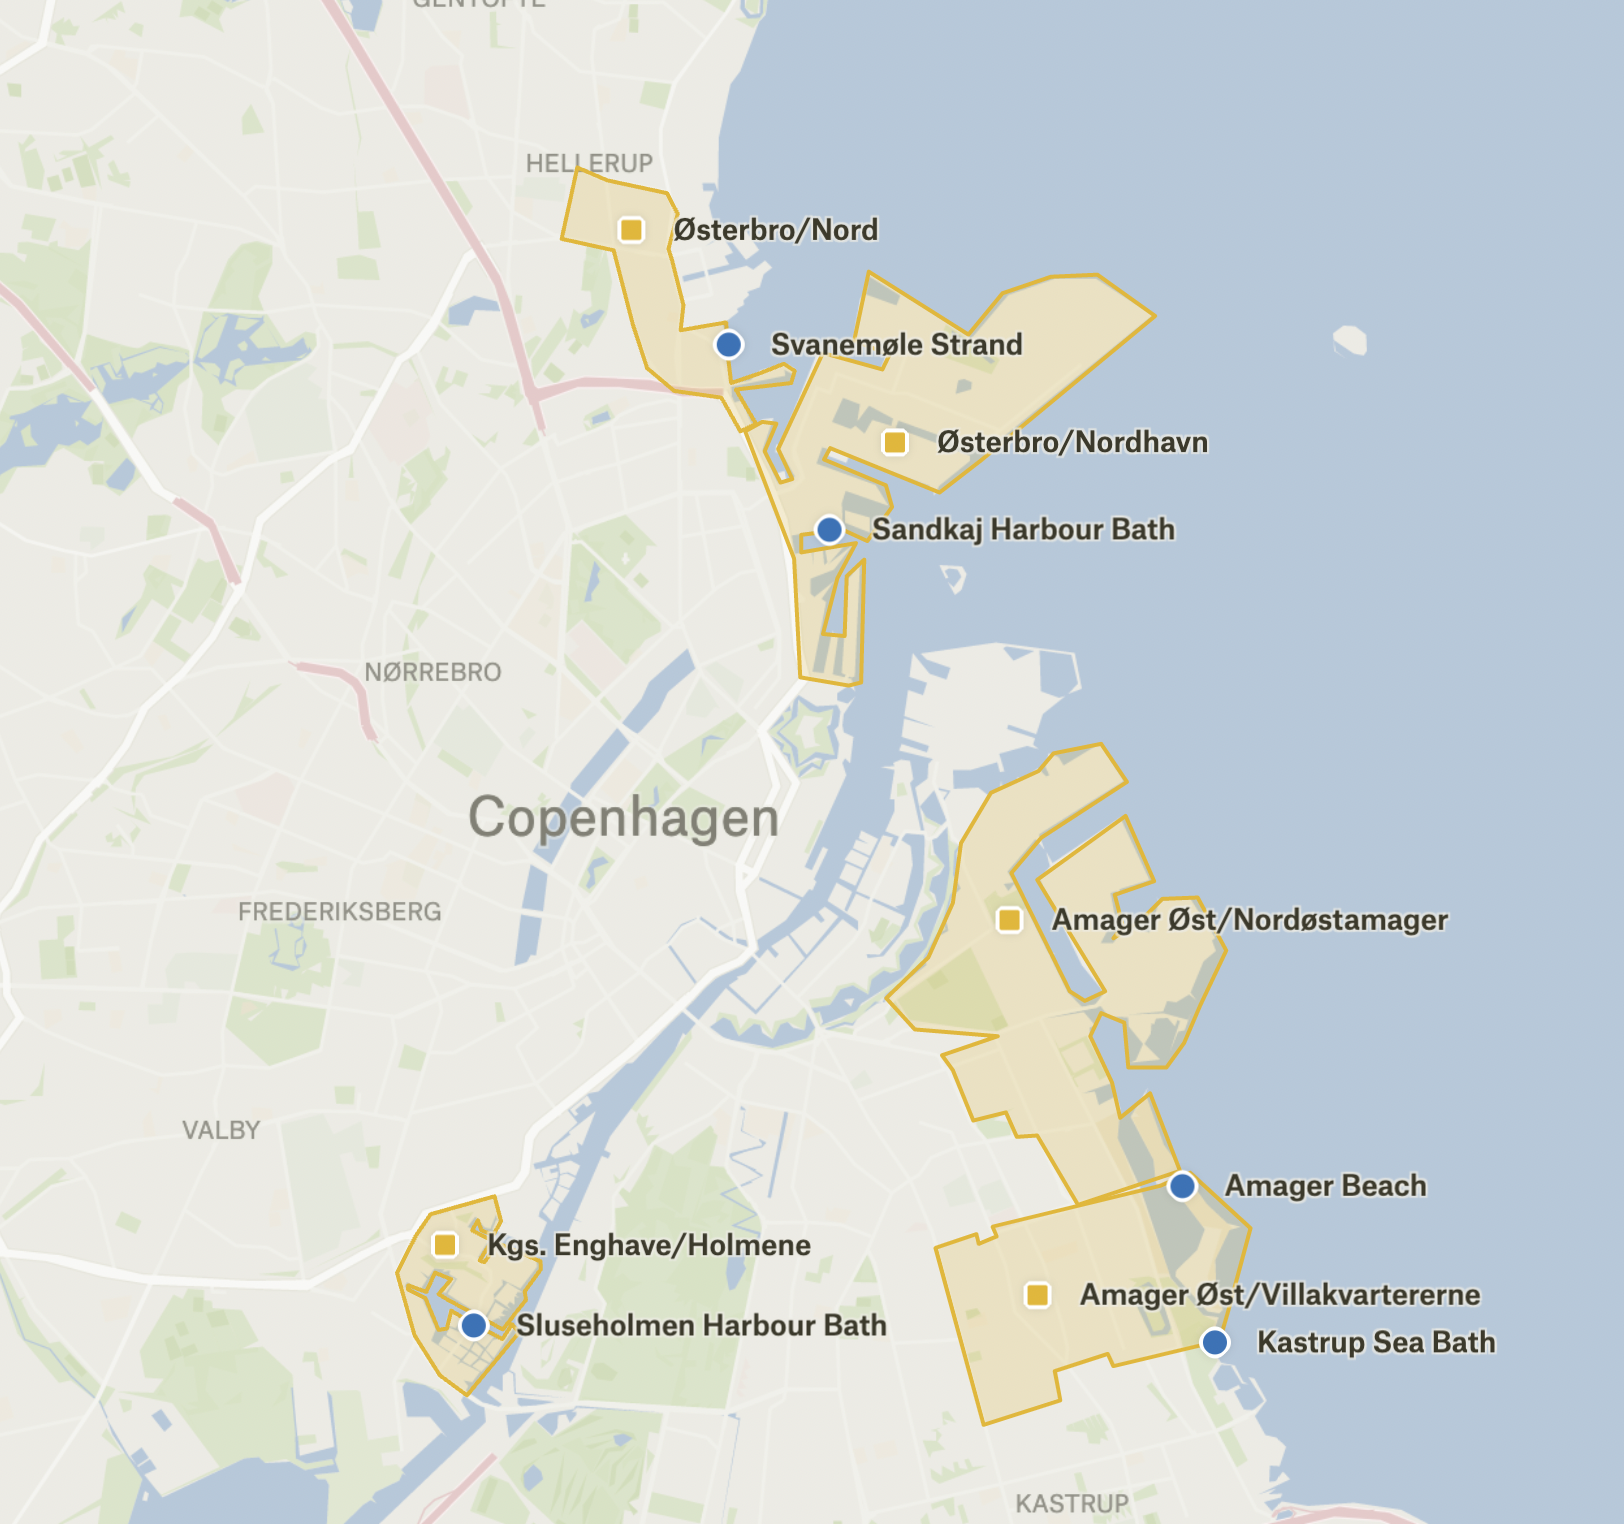
\includegraphics[width=\textwidth]{copenhagen_blue_spaces.png}
	\caption{A map of Copenhagen with the shortlisted blue spaces (blue dots) in their respective District/Neighbourhood (yellow areas labelled with yellow squares)}
\end{figure}


\begin{comment}

\bisection{Environmental justice}
Environmental justice (EJ) provides a lens through which to understand social and environmental inequalities related to blue spaces. By bringing together social and environmental concerns, the environmental justice paradigm advocates for the equal access to the benefits offered by natural spaces; and, in turn, sharing environmental burdens. 
EJ is traditionally broken down into three dimensions: distributional justice, procedural justice, and recognition justice \parencite{todo:cite schlosberg}.
% explain that this is most relevant for my research...
Recognising the experience of those who do not fit into the `norm' also means acknowledging that some practices take place in the private and not public sphere, because of historical racial, sexist, ethnic discrimination. For example, women who disproportionally carry out domestic and care work have a different daily pattern which does not match that of the average 9-5 worker, and the spaces and mobility options should be adapted for them to reach blue spaces with ease. Or, they may feel more vulnerable and less safe in public, and prefer private spaces \parencite{wessells2014urban}. How can blue spaces be inclusive of a diversity of people, carrying out a diversity of activities at all times of the day, week, or year? 
% Language like ``place-disruption'' and ``place-protection'' can promote mutual understanding, and avoid privileging the values of the mainstream over the values of marginalised communities \parencite{toomey2021place}.
% To understand injustices suffered by those who do not fit in to the white, heteronormative, upper-class cateogy, Anguelovski et al. (\citeyear{anguelovski2020expanding}) propose two goals to advance the concept of justice: 1, uncovering the material and immaterial power, and 2, advancing new principles for equity in urban greening. - TODO explain these concepts?
% TODO --> Mention similarity to Hong Kong, and perhaps limitations of that study
Ultimately, unequal access to blue space is an environmental injustice and this framework will lead my research. Environmental justice is a multi-faceted concept which brings together social and environmental concerns. Amongst other things, it advocates for the equitable access to environmental benefits. The dimension of justice that I will focus on is recognition. Recognition justice deals with people and groups’ perceptions, values and preferences which may influence the ways in which they interact, or not, with a blue space \parencite{anguelovski2020expanding}.
\end{comment}

\section{Timeline and feasibility}

UBS visits are highly dependent on the weather, meaning that people spend much more time at the water in summer than winter. Therefore, I aim to collect my data starting in August and going up to November. This should allow me to capture a wide range of users and uses, especially given that swimming culture is big in Denmark and people do use UBS all year. I will also be collecting data at different times of the day (morning, afternoon, evening) and week (weekdays, weekend, holidays).

\begin{ganttchart}[
hgrid,
vgrid,
expand chart=\textwidth,
time slot format=isodate-yearmonth,
time slot unit=month
]{2022-03}{2023-06}
\gantttitlecalendar{year, month} \\
\ganttbar{Thesis proposal}{2022-03}{2022-06} \\
\ganttbar{Create collection guides}{2022-07}{2022-07} \\
\ganttbar{Data collection}{2022-08}{2022-11} \\
\ganttbar{Literature review}{2022-09}{2022-11} \\
\ganttbar{Data analysis}{2022-12}{2023-03} \\
\ganttbar{Writing report}{2023-03}{2023-06} \\
\ganttmilestone{Thesis defence}{2023-06}
\end{ganttchart}

\section{Conclusion}

\printbibliography

\end{document}

%%%%%%%%%%%%%%%%%%%%%%%%%%%%%%%%%%%%
%				COMMENTS
%%%%%%%%%%%%%%%%%%%%%%%%%%%%%%%%%%%%

\begin{comment}
THESIS NOTES

Limitations:
- Observations done by a single person may not be reliable, would be more reliable and richer if conducted by 2 researchers who could debrief their observations and discuss their interpretations
\end{comment}
